\documentclass[11pt]{article}

\usepackage[letterpaper, total={6.5in, 8.5in}]{geometry}
\usepackage{fancyhdr}
\usepackage{float}
\usepackage{url}
\usepackage{graphicx}
\usepackage{bibentry}
\nobibliography*
\graphicspath{ {../Figures/} }

\title{CSCE 689 Winter 2016: Project Literature Review}
\author{Paul Jordan and Chip Van Patten}

\pagestyle{fancy}
\makeatletter
\let\runauthor\@author
\let\runtitle\@title
\makeatother
\lhead{\runauthor}
\rhead{\runtitle}

\begin{document}
\maketitle
\section{Concept Diagram} 
% with short description no more than three sentences
\begin{figure}[H]
  \centering
  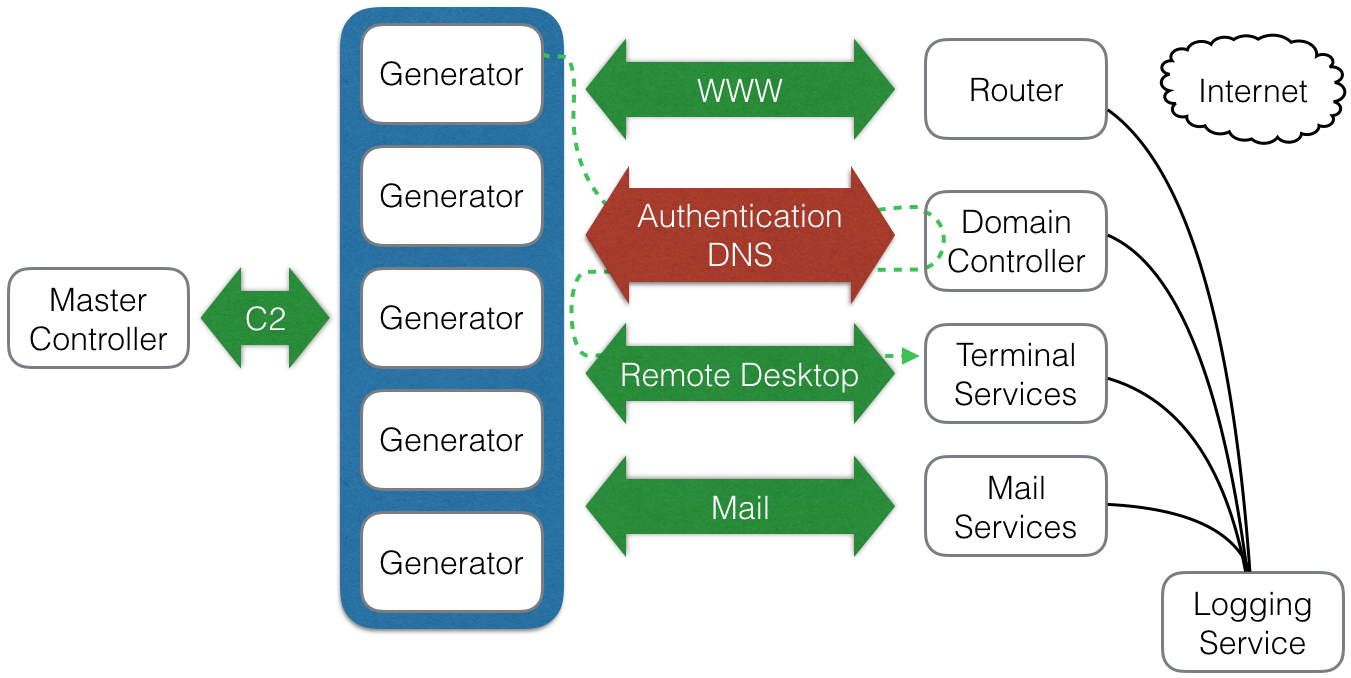
\includegraphics[width=6in]{ConceptDiagram}
  \caption[Concept Diagram]{How each generated traffic type is routed.  Log events are offloaded to logging service for
  further analysis.}
  \label{fig:conceptDiagram}
\end{figure}


\section{Potential Publication Opportunities} 
% Need at least three (name, place, abstract due date, paper due date, conf dates,
% any additional info
\begin{itemize}
\item{2016 IEEE International Conference on Software Quality, Reliability \&
Security (QRS16): Vienna, Austria, 1-3 August 2016.  Paper due date 25 March 2016
(Fast Track Abstract only submissions due 29 April 2016).
\url{http://paris.utdallas.edu/qrs16/}.}
\item{2016 ACM Special Interest Group on Data Communication (SIGCOMM) -
Internet QoE Workshop: Salvador, Brazil, 22-26 August 2016.  Paper registration
18 March, submission 25 March 2016.
\url{http://conferences.sigcomm.org/sigcomm/2016/qoe.php}.}
\item{2016 International Conference on Simulation and Modeling Methodologies,
Technologies and Applications (SIMULTECH 2016): Lisbon, Portugal, 29 - 31 July 2015.
Papers due 8 March 2016. \url{http://www.simultech.org/Home.aspx}.}
\end{itemize}

% ------------------------ Actual Lit Review Here -----------------------------
% Identify the problem, intuition/approach, solution and evaluation in several
% paragraphs. After summarizing the article in this way, provide your critique,
% providing 2 weaknesses, 2 strengths and 2 extensions that you could make to
% the paper. You can identify more than 2 if you want. Only use technical
% strengths/weaknesses or extensions (i.e. this paper read well, this part was
% poorly written/presented, the figures were hard to understand).
\newpage
\section{Prediction of failure occurrence time based on system log message
pattern learning}
\paragraph{Paper bibliographic information:}
\bibentry{sonoda2012}
% Paul.
\paragraph{Summary:}  The authors of this paper address the issue of network
device failure prediction in a cloud infrastructure environment.  The problem
presented is that while many machine learning based failure prediction methods
have been developed, none of them work sufficiently well enough to predict
failure in a distributed environment.  Further, if one is able to accurately
predict failure in a distributed environment via a machine learning algorithm,
a system update or network topology change can render that predictor useless.
Their solution is to have a predictor continuously learn through Bayesian
inference what failure looks like.  The authors then evaluated their new
approach against log messages obtained from an actual system and were able to
predict two types of failures that existed in the training data with an average
precision of approximately 0.8 and an average recall of approximately 0.9.\\

The authors' reported results compare favorably to some existing approaches
seen in~\cite{salfnerSurvey}.  Their overall contribution sets the stage for
research done since this papers publication which proves this method.
Unfortunately, the approach presented in this paper does require at least one
failure actually occur to be effective.  This is a weakness in many of the
machine learning based prediction techniques in literature.

\paragraph{Strengths:}  I believe the authors of this paper did an excellent
job documenting each aspect of their experiment with enough detail to allow for
a replication.  I also think that they did a good job outlining where the work
should go after this.  Finally, having real failure data available as the
authors did, to train their predictor is not easy and definitely makes the
results more compelling.

\paragraph{Weaknesses:}  Unfortunately, I don't believe the authors did a very
good job explaining how or why their method would be effective in adapting to
changing environments.  I also believe that they could have (as they pointed
out) tested their approach against a live network instead of static data or
looked for other types of failure within the training data.  Ultimately, I
think the main weakness in this paper was the static data used to train the
predictor which consequently happens to be one of its strengths.  This
contradiction leads to an interesting extension of being able to replace static
failure data with realistic simulated data.

\paragraph{Extensions:}  I think that a natural extension of this work would be
to do as the authors suggested and test this method on a live system and
compare it to another method.  I also think a good extension would be to
attempt to identify other types of failure instead of the two that were
selected for this experiment.
% End Paul.

\newpage
\section{Design of Software Network Traffic Generator}
% Chip.
\paragraph{Paper bibliographic information:}
\bibentry{zach2013}
\paragraph{Summary:}  The authors of this paper attempt to address a lack of network traffic generators which interact with pre-existing servers (WWW, mail, and multimedia) in a two-way manner.  They compare five open-source traffic generators that are either flow- or packet-level generators, but are all one-way in the traffic they generate (they simply send traffic to a receiver and do not care about getting a response).\\ 

The authors' proposed solution, uninspiringly nicknamed, NTG (short for \textbf{n}etwork \textbf{t}raffic \textbf{g}enerator), attempts to bridge the gap left by one-way traffic generators by connecting to a server and waiting for a response prior to sending more packets.  It is composed of five components: (1) a controller or management server which issues the list of commands to the (2) senders, one or more (3) servers that respond to senders' requests, a (4) packet capture server which records the traffic on the network, and a (4) statistics server which receives packet captures from (4).  At the time of publishing, NTG supports five protocols: ICMP, HTTP, POP3, SMTP, and RTP and assumes that, for each protocol, there is a pre-existing server waiting to respond.  The authors explain how to setup NTG and perform an experiment demonstrating its ability to produce HTTP and RTP flows to two different servers.  They then present the results gathered using the embedded tcpdump.

\paragraph{Strengths:} The authors did a good job considering bandwidth utilization issues that might occur when the management server is operating in-band with the network being tested and offer built-in support for out-of-band management links.  They also do a good job of explaining how NTG interacts with both a test network and each of the individual components so that reproducing the setup would not be too difficult. 

\paragraph{Weaknesses:}  The authors fail to convince the reader that their solution is any better than the current offering of traffic generators.  There is no feature or performance comparison to any other generator, even the ones mentioned in their paper.  Their test, as related in the paper, is difficult to follow (and would therefore be difficult to reproduce) and only included two of their supported protocols.  Again, they did not compare their results to the performances of any of the other network traffic generators, but more disappointing, they did not compare their results to actual network traffic generated by users on a live network.

\paragraph{Extensions:}  One extension to the proposed solution would be to incorporate more protocols and traffic that authenticates to a domain controller (for use in Enterprise networks).  Furthermore, testing the solution against other similar tools would be beneficial in proving the capability of the proposed tool.

% End Chip.

\newpage
\section{Adaptive Failure Prediction for Computer Systems: a Framework and a
Case Study}
% Paul.
\paragraph{Paper bibliographic information:}
\bibentry{irrera2015}
\paragraph{Summary:}  In this paper, the authors present a solution to the
problem of having good machine learning based online failure prediction methods
and having them go unimplemented.  The claim is that while machine learning
algorithms while have become very effective tools in failure prediction based
on reported errors (or log messages), they are unfortunately susceptible to
underlying system changes.  As a result, every time a piece of software is
updated a predictor used on that system is at risk of becoming obsolete.
Retraining that predictor is often a labor intensive process and requires
access to real failures of that system which often times isn't available.  The
solution presented in this paper is a framework for automatically generating
failure data to automate the process of training machine learning based
predictor.\\

The framework is designed to clone a production machine in a virtual
environment after a system update.  After the clone is created, a load
generator is started to place the clone under load.  Next, the cloned system is
injected with software faults to accelerate the failure process.  The resulting
log messages are used to train a new predictor.  The new predictor is then
compared with the old and if it performs better, it replaces the old.

\paragraph{Strengths:}  The authors of this paper have done a great job
convincing the reader that their framework works as they have claimed it does.
By conducting a case study and presenting the results, there is little room for
doubt.  Another really interesting thing the authors have done is provide
evidence that virtualization and simulation do not have any negative effects on
the training of machine learning failure prediction methods.  This puts to rest
any concern that their approach may not work in a production environment.

\paragraph{Weaknesses:}  Unfortunately, replicating this experiment and
recreating the framework does not appear to be an easy task as the authors have
left out key details.  They have not included the parameters or any specific
details on two major components of the framework, the predictor, and the fault
injection tool.  Additionally, the authors could have done more to generalize
their approach.  The case study proves that the framework is viable under a
very specific set of circumstances, but could be shown to work under others
without much modification.

\paragraph{Extensions:}  A natural extension would be to generalize the
approach.  Implement the same experiment for a different system and see how it
performs.  Another obvious extension would be to swap out different modules in
the framework to see how well it performs.  For example, in the experiment
conducted in this paper, an SVM predictor is used.  The same experiment could
be conducted using a Semi-Hidden Markov Model or any one of the number of other
prediction techniques seen in~\cite{salfnerSurvey}.
% End Paul.

\newpage
\section{D-ITG Distributed Internet Traffic Generator}
% Chip.
\paragraph{Paper bibliographic information:}
\bibentry{Avallone2004}
\paragraph{Summary:}  This paper presents a solution to distributed network traffic generation.  The authors implemented a traffic generator that emulates various network protocols utilizing models for ``the inter departure time between packets and packet size stochastic processes''\cite{Avallone2004}.  Their tool is composed of four parts: (1) ITGSend sends traffic, (2) ITGRecv listens for traffic , and (3) ITGLog stores logs generated by (1) and (2), and (4) ITGManager which provides remote control of (1).  Traffic is generated using predefined probability distributions and models for such protocols as UDP, TCP, ICMP, DNS, Telnet, and VoIP.  Logging can be performed locally on ITGSend and ITGRecv, or by sending the logs to ITGLog.\\

The authors conclude by briefly detailing an experiment conducted using their tool to generate a 60 second UDP flow.  They provide analysis of their tool and compare it to the analysis of other traffic generators running the same experiment parameters.  Their future work includes developing D-ITG to run on additional platforms and implementing several other application layer protocols. 

\paragraph{Strengths:}  The authors do a decent job of providing a breakdown of each component of the tool and how they interact.  Another strength is the use of embedded models to set certain protocol parameters, thus abstracting them from the user, means the user does not have to enter those values manually. 

\paragraph{Weaknesses:}  The author's claim their tool performs the best because its received data rate is closest to the expected value, but they do not go into any detail about how the expected value is calculated or why said value should be expected.  Similarly, the details of the design of all but one of their experiments are left out of this paper.  Furthermore, very little background is given on the current state of network generators or why their tool is ground breaking.

\paragraph{Extensions:}  The solution could be further extended by allowing real traffic (either through a packet capture file or live network traffic monitoring) to be used for the traffic generation.  Additionally, implementing two-way traffic generation between ITGSend and ITGRecv would provide a more realistic traffic generation tool that would allow more practical analysis of a network to occur. 

% End Chip.

\newpage
\bibliography{../LoadGenerator}{}
\bibliographystyle{plain}

\end{document}
